%----------------------------------------
% Preamble to set up the document
%----------------------------------------
\documentclass{article}

% set up packages (you shouldn't need to touch this)
\usepackage{graphicx}  % required to insert images
\usepackage{hyperref}  % for hyperlinks
\usepackage[svgnames]{xcolor}  % to change hyperlink colors
\colorlet{linkcolour}{DarkBlue}
\hypersetup{colorlinks=true, linkcolor=linkcolour, citecolor=linkcolour, urlcolor=linkcolour,}

% Margins
\topmargin=-0.45in
\evensidemargin=0in
\oddsidemargin=0in
\textwidth=6.5in
\textheight=9.0in
\headsep=0.25in

% use a sans serif font
\renewcommand{\familydefault}{\sfdefault}

%----------------------------------------
% Step 1: Edit the lecture title
%----------------------------------------
\title{
Lecture 10: Classification & Networks  \\  % Lecture title
Modeling Social Data, Spring 2019 \\   % Course title
Columbia University                    % School
}

%----------------------------------------
% Step 2: Edit your name and the date
%----------------------------------------
\author{Brigid Lynch}                     % Scribe's name
\date{April 7, 2019}                % Lecture date

\begin{document}

\maketitle


%----------------------------------------
% Step 3:
% Rename uni.tex to match your uni,
% edit the filename accordingly below,
% and put your notes in this file
%----------------------------------------
%----------------------------------------
% Write your notes here
%----------------------------------------

%----------------------------------------
% Write your notes here
%----------------------------------------
\section{Introduction}
In  this lecture we'll finish going over classification and begin our discussion on networks. Namely we will look at more subtle aspects of classification such as the difference between logistic regression and linear regression and why one may be preferable. Later we'll do some coding which is where the R code will come in handy, looking at how we can use ggplot to think critically about what our classification models are saying. 

\section{Classification as Regression?}
\begin{equation}
   y\subseteq \{0,1\} y\subseteq R 
\end{equation}
Recall from last time Logistic Regression: 
\begin{equation}
    \log\frac{p}{1-p}=w\cdot x
\end{equation}
\begin{equation}
    L=\prod_{i=i} p_i^{y_i}(1-p_i)^{1-y_i}
\end{equation}

What if we just used linear regression to predict, something simple such as gender based on height? 
\begin{figure}[ht]
  \begin{center}
 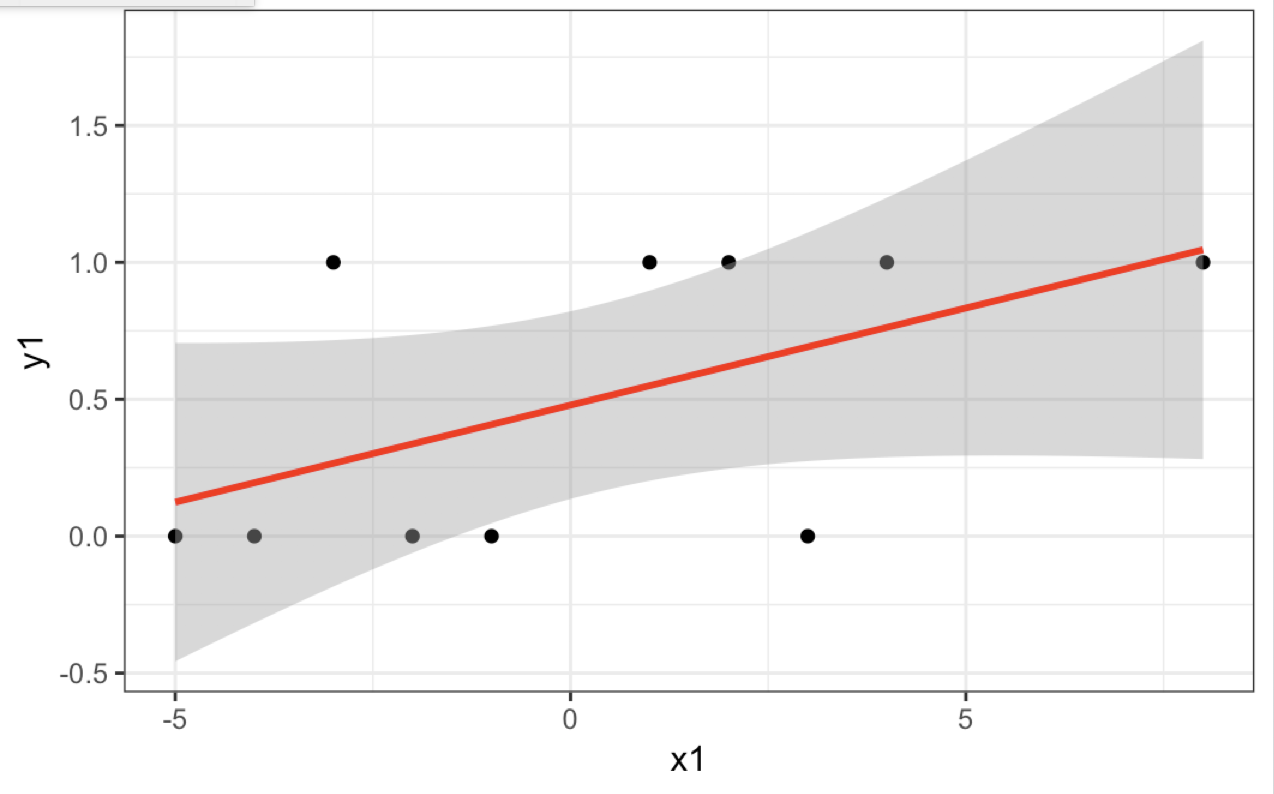
\includegraphics[width=0.3\textwidth]{lm2.png}
 \caption{The points represent height and gender (1 being male 0 being female and x representing height), the line is the regression line}
 \end{center}
 \end{figure}
 
 Since regression won't just be predicting 0 or 1, you're error rate may be incorrectly penalizing you, causing for an inaccurate line. Look at the graph, although line  values above y=1 are technically you will still get an error of y-1. Logistic regression prevents this. 


\section{Reading Regression Tables}
\begin{figure}[ht]
  \begin{center}
    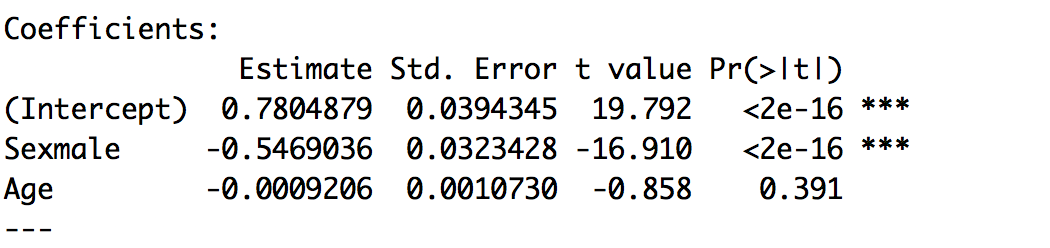
\includegraphics[width=0.5\textwidth]{logregesstable.png}
    \caption{ The output for a logistic regression table from the glm() function 
     }
    \label{fig:example_figure}
  \end{center}
\end{figure}
The key here is to remember that these are logistic regression coefficients and therefore one must do a transformation on all of these values (p being the different estimates):
\begin{equation}
    \frac{1}{1+\exp(-p}
\end{equation}
Examples: 
Likelihood of a 20 year old male surviving: (recall that .009 means for each year your likelihood of survival decreases) 
\begin{equation}
    \frac{1}{1+\exp(-.74204-.546-.009*20)}
\end{equation}
\begin{itemize}
    \item What does the Estimate,Intercept value mean? 
    \begin{itemize}
        \item The Likelihood of a 0 year old female surviving
    \end{itemize}
    \item This is why using predict() is useful, these coefficients are difficult to interpret 
\end{itemize}
We also looked at graphically examining predictions with ggplot
\begin{itemize}
    \item Emphasized bin size when looking at results
    \item ex: if you have less data points for 80 year olds than for 50 year olds then you should consider that when looking at your prediction results
\end{itemize}

\section{History of Networks}
Main idea of Networks: things are not completely independent! 
\begin{itemize}
  \item 1930s: Relationships as Networks,socio-grams first network diagrams,big deal NYT headline, examined runaway girls through a school social network (Moreno) 
  \item 1960s: Random graph theory:
  \begin{equation}
      p > \frac{(1+\epsilon)\ln_n }{n}
  \end{equation}
  \item 1970s: Clustering weak ties, theories motivated by intuition and smaller data sets 
  \begin{itemize}
  \item  Granovetter, The Strength of Weak Ties:"The degree of overlap of two individuals' friendship networks varies directly with the strength of their tie to one another"  Relationship exists and matters! 
  \item Forbidden Triad: Mutual friends are connected in strong relationships 
  \item Also examined whether one finds jobs through strong/weak ties, without weak ties strong groups would not relate to one another. 
   \item Cumulative advantage: de Solla Price, looked at citations of other academic papers, citations are highly concentrated among popular papers and then a "long tail" of lesser known papers  
  \end{itemize}
  \item 90s: internet, got a lot more data! Less interview based 
  \begin{itemize}
      \item  Small-world networks Watts and Strogatz, used probability and randomness to prove features of small-world networks 
      \clearpage
      \begin{figure}[ht]
  \begin{center}
    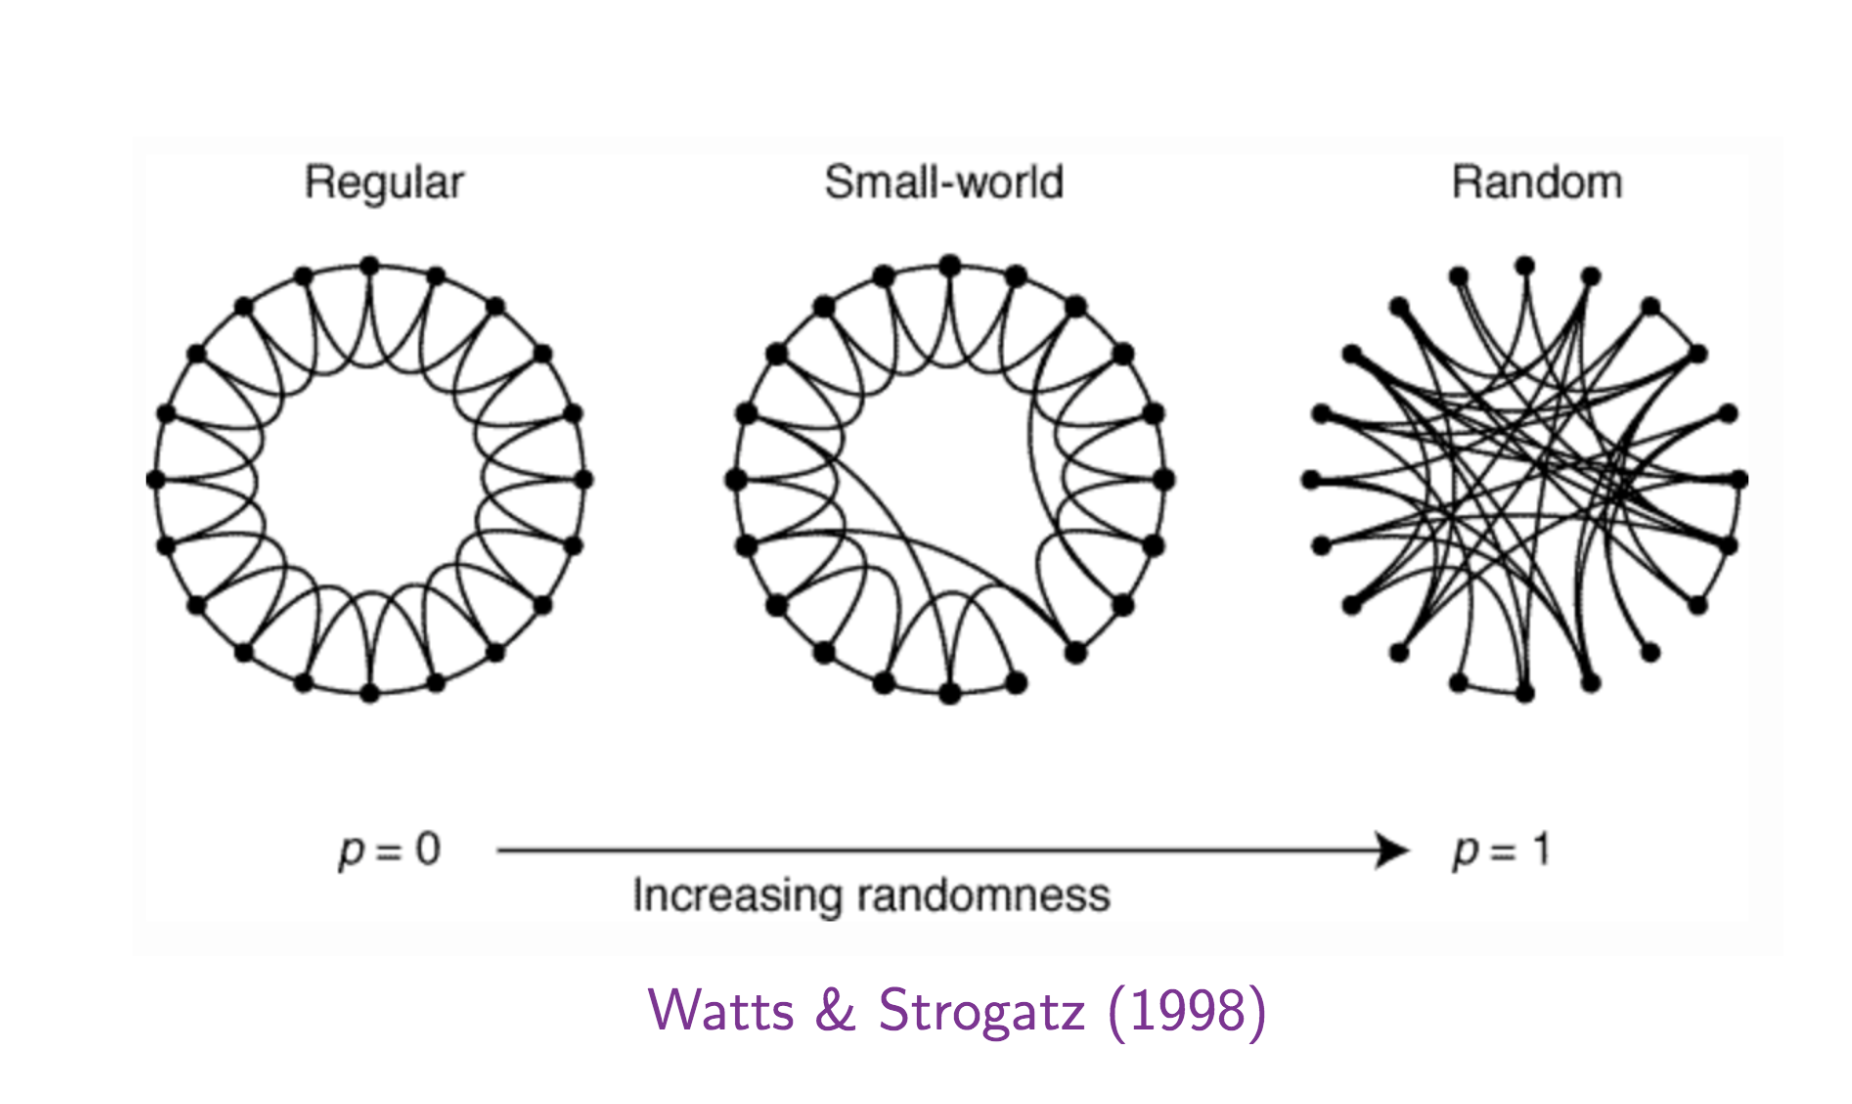
\includegraphics[width=0.5\textwidth]{smallworld.png}
    \caption{(From MSD Lecture 10 Slides) 
     }
    \label{fig:example_figure}
  \end{center}
\end{figure}
  \end{itemize}
  \item 2000s: Homophily, contagion and all that
  \begin{itemize}
      \item Adamic and Glance, looked at political viewpoints in blogposts and connections based on political orientation
      \item homophily: because you are similar you are friends
      \item contagion: because you are friends you are similar 
      \item Attempts to figure out which is the cause 
  \end{itemize}
\end{itemize}
\section{ Types of Networks}
Useful for many different types of data
\begin{itemize}
    \item Social Networks (Facebook)
    \item Information Networks (web) 
    \item Activity networks (email)
    \item Biological networks (protein interactions)
    \item Geographical networks (roads) 
\end{itemize}
There are also many different levels of abstraction for representing networks.(Directed, weighted, metadata). They can also vary depending on how detailed you want your representation to be. 

Which Network? Imagine a person's Facebook: 
\begin{itemize}
    \item ego network: person in middle all friends represented
    \item Maintained relationships: friends that actually interact
    \item One way communications
    \item Mutual communications 
\end{itemize}
Important: 
\begin{itemize}
    \item What is the network?
    \item What are you counting?
    \item What are you encoding?
    \item *Simple is often better, don't get too crazy 
\end{itemize}
\clearpage
\section{Adjacency Matrix}
\begin{figure}[ht]
  \begin{center}
    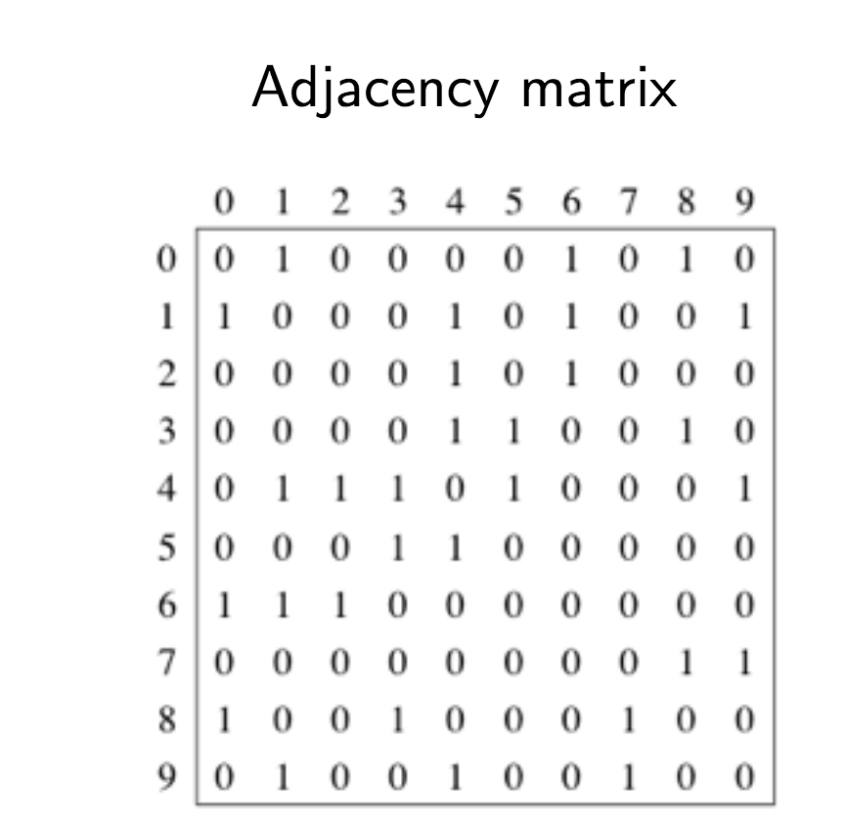
\includegraphics[width=0.5\textwidth]{matrix.png}
    \caption{(From MSD Lecture 10 Slides) 
     }
    \label{fig:example_figure}
  \end{center}
\end{figure}

 Time complexity if there is an edge: constant (index by row and column), find neighbors O(n), also good for linear algebra
 
\section{Adjacency list} 
\begin{itemize}
    \item  Good for graph transveral checking neighbors and going through the graph.
    \item Time complexity to check if an edge exists: O(average degree)) 
\end{itemize}


\section{Descriptive statistics}
\begin{itemize}
    \item Degree: How many connections does a node have?
    \item Path length: Shortest path between two nodes?
    \item Clustering: How many friends of friends are also friends?
    \item Components: How many disconnected parts does the network have? 
\end{itemize}





\end{document}

%%% Local Variables:
%%% mode: latex
%%% TeX-master: t
%%% End:
